\documentclass{standalone}
\usepackage{tikz}
\usetikzlibrary{positioning}

\begin{document}
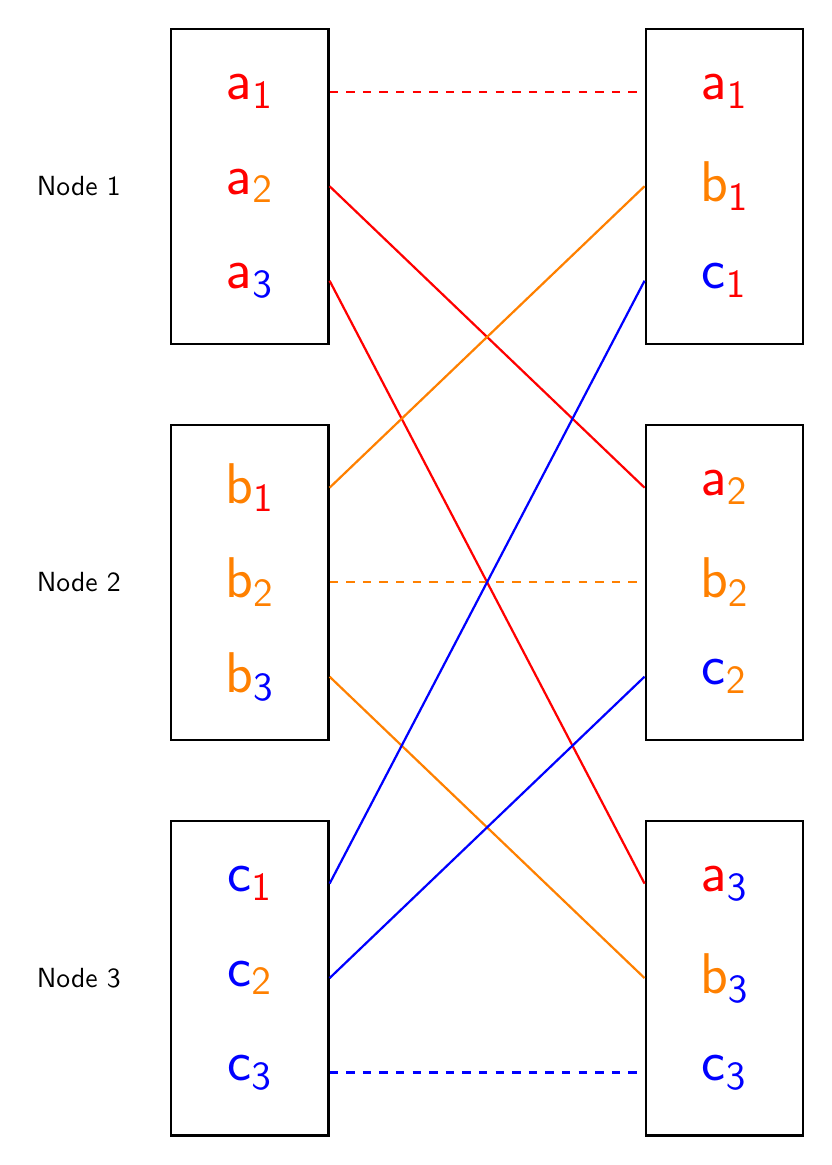
\begin{tikzpicture}[
    node distance=1cm,
    every node/.style={font=\sffamily},
    box/.style={draw, thick, minimum width=2cm, minimum height=4cm, align=center},
    element/.style={minimum height=0.4cm, align=center, font=\huge\sffamily}
]

% 左侧节点组
\node[box] (left1) {};
\node[box, below=of left1] (left2) {};
\node[box, below=of left2] (left3) {};

% 右侧节点组
\node[box, right=4cm of left1] (right1) {};
\node[box, below=of right1] (right2) {};
\node[box, below=of right2] (right3) {};

% 左侧节点内容
\node[element] at ([yshift=1.2cm]left1.center) {\color{red}a\textsubscript{\color{red}1}};
\node[element] at (left1.center) {\color{red}a\textsubscript{\color{orange}2}};
\node[element] at ([yshift=-1.2cm]left1.center) {\color{red}a\textsubscript{\color{blue}3}};

\node[element] at ([yshift=1.2cm]left2.center) {\color{orange}b\textsubscript{\color{red}1}};
\node[element] at (left2.center) {\color{orange}b\textsubscript{\color{orange}2}};
\node[element] at ([yshift=-1.2cm]left2.center) {\color{orange}b\textsubscript{\color{blue}3}};

\node[element] at ([yshift=1.2cm]left3.center) {\color{blue}c\textsubscript{\color{red}1}};
\node[element] at (left3.center) {\color{blue}c\textsubscript{\color{orange}2}};
\node[element] at ([yshift=-1.2cm]left3.center) {\color{blue}c\textsubscript{\color{blue}3}};

% 右侧节点内容
\node[element] at ([yshift=1.2cm]right1.center) {\color{red}a\textsubscript{\color{red}1}};
\node[element] at (right1.center) {\color{orange}b\textsubscript{\color{red}1}};
\node[element] at ([yshift=-1.2cm]right1.center) {\color{blue}c\textsubscript{\color{red}1}};

\node[element] at ([yshift=1.2cm]right2.center) {\color{red}a\textsubscript{\color{orange}2}};
\node[element] at (right2.center) {\color{orange}b\textsubscript{\color{orange}2}};
\node[element] at ([yshift=-1.2cm]right2.center) {\color{blue}c\textsubscript{\color{orange}2}};

\node[element] at ([yshift=1.2cm]right3.center) {\color{red}a\textsubscript{\color{blue}3}};
\node[element] at (right3.center) {\color{orange}b\textsubscript{\color{blue}3}};
\node[element] at ([yshift=-1.2cm]right3.center) {\color{blue}c\textsubscript{\color{blue}3}};

% 节点标签
\node[left=0.5cm of left1] {Node 1};
\node[left=0.5cm of left2] {Node 2};
\node[left=0.5cm of left3] {Node 3};

% 连接线
% 从左侧第一个节点出发的线
\draw[red, thick, dashed] ([yshift=1.2cm]left1.east) -- ([yshift=1.2cm]right1.west);
\draw[red, thick] (left1.east) -- ([yshift=1.2cm]right2.west);
\draw[red, thick] ([yshift=-1.2cm]left1.east) -- ([yshift=1.2cm]right3.west);

% 从左侧第二个节点出发的线
\draw[orange, thick] ([yshift=1.2cm]left2.east) -- (right1.west);
\draw[orange, thick, dashed] (left2.east) -- (right2.west);
\draw[orange, thick] ([yshift=-1.2cm]left2.east) -- (right3.west);

% 从左侧第三个节点出发的线
\draw[blue, thick] ([yshift=1.2cm]left3.east) -- ([yshift=-1.2cm]right1.west);
\draw[blue, thick] (left3.east) -- ([yshift=-1.2cm]right2.west);
\draw[blue, thick, dashed] ([yshift=-1.2cm]left3.east) -- ([yshift=-1.2cm]right3.west);

\end{tikzpicture}
\end{document}